%
% File: chap02.tex
% Author: ta16969
% Description: !!!!!!!!!.
%
\let\textcircled=\pgftextcircled
\chapter{TEL \& Modern Pedagogy Strategies}
\label{chap:TEL and Modern Pedagogical Strategies}


\initial{T}he chapter introduces the multi-cognate area of pedagogy \& TEL. By creating an understanding of relevant learning methods, pedagogies and introducing TEL modalities, the surmised rationale for the modal, creative and technical design of Artemis is deduced.

\section{Context : Understanding Modern Pedagogies, Learning Methodologies and TEL}

As the title suggests, the objective of this section is to introduce the idea of modern pedagogies and learning methodologies. It begins by explaining the contextual  and practical relevance of understanding the aforementioned to develop the design of a TEL solution, so that it is genuinely fit for purpose. It then moves on to understanding the shortcomings of  a traditional pedagogy and creates the underlying rationale for adopting modern pedagogies and learning methodologies, to effectively utilise TEL solutions such as Artemis. Finally the section explores which pedagogy and associated learning methodology is the best for adopting a TEL solution, to inspire and explain the creative design aspects of Artemis.

\label{sec:sec01}
\subsection{TEL a Silver Bullet? The Implications of Pedagogy on Product Design}
\label{subsec:subsec01}

There is a thematic perception across non-academic literature that adopting a TEL solution is effectively a \textbf{stand alone silver bullet} remedy for improved learning objectives and resource consumption. This perspective oversimplifies and ignores the nuances of a TEL solution's design compatibility with pedagogies and learning methodologies \cite{RickReis,Means2009,Team2008,Gordon2014,Burge2011}. This compatibility or incompatibility has an an \textit{inevitable} impact on the success of the TEL solution upon deployment i.e. the success of stakeholder adoption \cite{Mahamuni2015} or likelihood of improved learning and teaching outcomes \cite{RickReis,Means2009,Team2008}.

A \textbf{relevant example} to illustrate  and underline the importance of the relationship between user pedagogy, learning methodology and a TEL solution exists in the environment that Artemis is to be deployed i.e. at the UoB. Preliminary introductory meetings with the TELED department and UoB faculty has revealed that technically satisfactory and functional TEL solutions, have suffered from incompatibility with user pedagogies, lack of interest from instructors themselves, negative user perceptions (seemingly rife in the CS department at the UoB as per both stakeholders) and a resultant failure in the adoption of relevant TEL solutions. Instructors in particular when questioned about the lack of adoption almost unanimously cite a poor UX/UI and above all a lack of genuine utility towards learning and teaching objectives.

Interestingly literature exists to rationalise instructor and user perception from this perspective; a poorly designed UX and/or immaterial errors in the UI deteriorate the \textit{Web Credibility} and \textit{persuasiveness} of a technology, therefore resulting in lack of adoption (See Chapter \textbf{\ref{persuasiveWebDesignStart}} for details). 

Literature  implies that TEL solutions reliant on self directed learning methodologies \& pedagogies are undesirable for UK institutions such as the UoB because of their negative policy implications such as deterioration in ranking and resultant deterioration in access to finance \cite{Gordon2014}. It can be reasoned that perhaps Artemis should not be modelled as a self directed TEL solution as this may result in outright rejection from the UoB administration.

However more importantly within the context of TEL and pedagogy compatibility; despite the short comings of traditional instructor lead class room techniques,  the presumption that  completely substituting them in favour of \textit{self-directed} and \textit{drop-in} e-learning programmes because the latter are the  best alternative replacement seems statistically incorrect \cite{RickReis,Team2008}. Research based evidence suggests that contingent on the choice and implementation of a pedagogy,  TEL solutions adopted at academic institutions may end up \textbf{equivalent} if not \textbf{inferior} than traditional teaching   methodologies, within the scope of specific learning metrics \cite{RickReis,Means2009,Team2008}. This evidence is further considered in detail, along with it's implication on the design of Artemis in Chapter \textbf{\ref{embeddingBestPracticePedagogy}}. At this stage it suffices to conclude that an incompatibility in pedagogy and TEL solution design (such as a wholey self directed one) can result in unexpected costs and compromised in learning as well as administrative objectives, as opposed to advantages. 

The aforementioned conclusion has a strong implication for Artemis; \textbf{obliviousness} towards pedagogy (as well as other aspects explored later such as Web Credibility to note one of many) can result in \textbf{outright failure after deployment}, justifying the need for an underlying design rationale and the preliminary research carried out in these early chapters of the report to inspire Artemis during development through value sensitive design principles \cite{Mahamuni2015}.

Another common presumption that TEL saves resources is not necessarily true \cite{Gordon2014,Hackelbusch2007}. Avoiding deviation from the scope it is reasoned that within the context of this project the proposed TEL solution should at the very least endeavour to achieve value for money via improved learning outcomes. An extensive detailed review of stakeholders and other design values not discussed in this report, whilst genuinely prudent for a holistic design solution, would be beyond the reasonable project constraints and have been excluded for the most part.



\label{sec:sec01}
\subsection{Towards TEL Compatible Pedagogies: Why Depart from Traditional Pedagogy and Learning ?}
\label{subsec:subsec01}

Attitudes towards teaching practices in the UK that progressively adopt alternatives to traditional instructor facing, classroom based curriculum deliveries seem to have matured in recent years \cite{Jessica2012,CinYeeHoo,Stuart2014}; Particularly in CS curriculum's where an appetite for adopting technology enhanced learning tools and associated teaching solutions seems higher, in a wide range of academic institutions, particularly for teaching  foundation  skills such as programming \cite{Ibanez2014,Serrano-Laguna2015,Bittencourt2015,Chigona2008,CinYeeHoo,Jessica2012,Stuart2014}. The cause for the growing importance of teaching CS skills is irrelevant to the scope of this study, but it seems reasonable to assume  maturing technology markets and  a resultant market appetite for technically skilled labour \cite{CinYeeHoo,Stuart2014,Jessica2012}.

However despite changing perceptions and a growing appetite for utilising modern pedagogies for teaching at various level \cite{Chigona2008,CinYeeHoo}, existing scarce traditional teaching resources are subject to claims of stress, scarcity and  resultant perceptions of inadequacy \cite{CinYeeHoo}. The reasons for the scarcity are admittedly almost certainly politicised and murky \cite{Stuart2014,CinYeeHoo,Jessica2012}, however they do imply a tentative relationship with the inflexibility of traditional pedagogies.

The implication of a resultant scarcity or shortage  of limited traditional teaching resources due to the choice of a traditional pedagogy can be drawn; Irrespective of academic institution these shortages are likely to be commercially undesirable and may cause consequent deterioration or at worst outright failures of intended pedagogical strategies and resultant learning objectives \cite{Gordon2014,CinYeeHoo,Stuart2014}. Resources dedicated towards introductory programmings courses such as those at UoB are usually scarce to begin with \cite{Chigona2008}, thus there is an appetite to attempt substituting or complimenting these methodologies with TEL to try and alleviate commercial and pedagogical shortcomings, in favour of improved learning outcomes \cite{Chigona2008,Hackelbusch2007,Serrano-Laguna2015,Bittencourt2015,RickReis,Chat2014}.

Indeed when the difficulties faced by the UoB CS department within the context of W-0 are compared with shortcoming of traditional pedagogies, the rationale for a TEL solution such as Artemis seems reasonable. UoB's shortcomings likely caused compromised learning and administrative objectives and a wastage of limited teaching resources. As introductory programming courses at universities and colleges such as the UoB are resource intensive \cite{Chigona2008}, a TEL solution such as Artemis may offer scope for improved learning outcomes when teaching programming \cite{Ibanez2014,Bittencourt2015,Serrano-Laguna2015} and efficiency in utilisation of resources.

In summary to conclude; within the context of introductory programming, CS education and commercial rationale  an appetite for adopting modern pedagogies that use TEL seems reasonable and not without merit. This is indicatively presented as underlying justification for undertaking the development of the Artemis project.


\label{sec:sec01}
\subsection{A Viable Alternative: Definition}
\label{subsec:subsec01}

From a strictly pedagogical and learning perspective it is reasoned, that any \textbf{sincerely viable alternative} solution to the shortcoming of a traditional and instructor lead class room teaching methodology would achieve at the very least achieve equivalent if not improved learning outcomes \cite{RickReis,Means2009}. 

Furthermore for this project resource savings exploring the commercial and the economic implications of implementing a TEL solution are deemed outside of scope, other than  abstract identification or incidental findings during the course of the report. Any commercial savings as a result of deploying the TEL tool are  deemed ancillary; For this project resource savings are to be interpreted as giving strategic flexibility to the instructor's pedagogy, towards the benefit of learning outcomes for students.



\label{sec:sec01}
\subsection{Blended Learning Approach}
\label{definingBlendedLearning}

The alternative approach to an instructor lead class room pedagogy lies in a \textit{blended/hybrid learning} methodology \cite{Means2009,RickReis,Gordon2014}. As figure 2.1 illustrates, "Blended learning aims to mix TEL with more traditional forms" \cite{Gordon2014}, where "form" implies instructor lead class room course deliveries \cite{RickReis,Means2009}.

% A single figure
\begin{figure}[H]
	\centering
	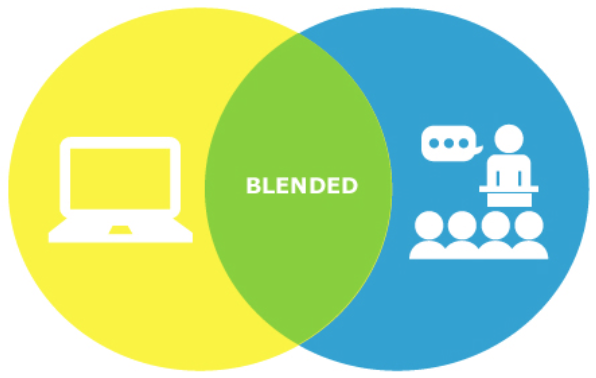
\includegraphics[height=0.35\textheight]{figures/blendedLearning}
	\mycaption[Blended Learning Infographic.]{Blended Learning Infographic. Figure reproduced from \cite{Gordon2014}.}
	\label{fig:Blended Learning}
\end{figure}

The precise definition of blended learning is poorly defined by academic sources \cite{Oliver2005}. This research wont attempt to define one, as the ambiguity in definitions does not seem problematic for the purposes of developing and implementing the relevant TEL solution. However for clarity in discussion and interpretation of relevant literature, it will usually imply the following ; "the integrated combination of traditional learning with web-based online approaches" \cite{Oliver2005}, whilst interchangeably applying alternative definitions that broadly imply \textit{blending a combination of different approaches with traditional instructor lead ones} \cite{Oliver2005,Sana2011}. Neither of these definitions are right or wrong (although the former is more relevant), and the interchangeable and ambiguous usage of key terminology such as "blended learning" seems rife and the norm in relevant literature\cite{Oliver2005,Sana2011}.

Interestingly despite a seemingly growing wealth of research that compares self-directed TEL, traditional instructor-lead methodologies and blended learning approaches implemented in various academic organisations, initial conclusions about which of these are superior are hard to draw due to ambiguous and conflicting results \cite{Means2009}. Extensive meta-analysis of such research \cite{RickReis,Means2009,Team2008} reveals that in most cases the  difficulty in drawing clear conclusions is attributable to different methodologies, as well as varying contextual interpretations of the definition of what qualifies as a blended learning or one of the alternative "pure" implementations .

It is tentatively reasoned based on the extensive meta-analysis of research on the subject \cite{Means2009,Team2008,RickReis}, that the previously discussed academic ambiguity (section \textbf{\ref{definingBlendedLearning}}) regarding the \textbf{poor definition of blended learning}, may contribute towards the difficulty in drawing conclusions in determining the best learning methodology. This is because murky academic definitions and interpretations may be the cause of various interpretations in the scope of research for the comparative studies \cite{Means2009,RickReis,Team2008} and give credence to the idiom \textit{comparing apples to oranges}.

Fortunately, an extensive meta-analysis of significant depth and scope by Murphy et al \cite{Means2009} on a large sample of comparitive research,  concluded that \textbf{collaborative} (instructor directed TEL solutions)  achieved learning and pedagogical results superior to those attained through independent, self-directed online learning \cite{RickReis} and instructor facing class room methodologies, a view corroborated by other  meta-analysis on relevant literature  \cite{Means2009,Team2008,RickReis}. Note the emphasis on an instructor lead pedagogy is not mutually exclusive of a blended pedagogy.

Therefore it is reasoned that the TEL solution to be developed for this project i.e. Artemis, should be an enabler for blended learning methodologies and associated pedagogies that are instructor lead; to yield the best learning outcomes.

\label{sec:sec01}
\subsection{Embedding Proven Best Practice in Design Criteria}
\label{embeddingBestPracticePedagogy}

Despite determining that a blended learning approach is the superior of the alternative learning methodologies for adopting TEL, it is important to note that effective adoption of a blended learning approach has caveats and nuances that need to be incorporated into the overall design of the TEL solution; in order to achieve the best possible learning outcomes. The following design consideration are hallmarks of blended learning methodologies that have demonstrated the best learning outcomes, when compared against other methodologies (blended or otherwise)\cite{Means2009,Team2008,RickReis}:


\begin{enumerate}

    \newpage

    \item \textbf{Instructor Directed Learning vs Self Directed Learning}:
    
    Self Directed Learning, as with most terminology in  the field seems to lack a unified definition \cite{OShea2003,Hiemstra2006}, which causes resultant difficulties in comparing research. Within the context of this study it refers to "Self Directed E-Learning", which may feature as part of a blended learning methodology. It is associated broadly with empowering students with the choice to define and control various aspects of their curriculum, learning process and methodology in isolation \cite{Hiemstra2006,Means2009,RickReis,Team2008} from traditional teaching environments. This approach does not yield the best learning outcomes out of the available alternatives and is rejected as a design choice for the TEL solution in this project \cite{RickReis,Team2008}. 
    
    Instead instructor directed online learning is deemed to be a more effective pedagogy in terms of favourable learning outcomes. As opposed to learning in isolation from the instructor, student's who receive tailored feedback and guidance  i.e. \textit{prompts} from the instructor \textbf{during} the learning process, benefit from more favourable learning outcomes as well as enhanced user engagement \cite{RickReis,Team2008,Means2009}.


    \item \textbf{Instructor Lead Resources Should be Adapted for the TEL solution}:
    
    The adaptation of instructional methodologies and course materials within the context of an online environment or TEL solution is evidenced as a hallmark of successfully adopted blended learning approaches in academic institutions \cite{Means2009,Team2008,RickReis}. This implies that pedagogies need to be adaptable towards the successful implementation of a TEL solution and blended learning methodologies, be it the instructions or learning material.
    
    Pedagogies that lack the flexibility to adapt instructions and material to TEL, are likely to deteriorate the efficacy and intended outcomes of a TEL solution or blended learning methodology \cite{RickReis,Team2008,Means2009}. This point naturally leads on to the next section of this chapter on a flexible pedagogy that can make the most of TEL solutions and instructor lead blended learning methodologies.
\end{enumerate}


Before concluding this section design implications from the aforementioned can be drawn and summarised for the purposes of developing a TEL solution for this project. \begin{enumerate}
    \item The ideal TEL solution that prioritises learning outcomes for W-0 should be an enabler for \textbf{instructor lead} blended learning and associated pedagogies.
    \item Artemis should also be an enabler for flexible adaptation of both instructions and course material.
\end{enumerate}


The next design criteria is do with how to embed  flexibility within the design of the TEL solution, whilst enabling  both instructor lead and adaptable delivery for a successful blended learning approach. The answer to this is designing the tool in a manner that it is synergistic with \textbf{ \textit{flexible pedagogies}} \cite{Gordon2014,Burge2011}; designed for utilising blended learning with TEL in a manner that encourages flexibility on specific aspects of learning, to ultimately benefit key stakeholders. This pedagogy is discussed in the next section and builds on from the rationale built thus far in this section.

Regarding \textbf{instructor directed learning}, the question arises; How can the practical flow of this  interaction be illustrated or incorporated within a TEL product? A potential answer lies in seeking design inspiration based on  \textit{participatory learning models} \cite{Yager1990,Yager2004}, using design inspiration from neural networks and AI  that are analagous to optimising human interaction for learning, implemented via a social network \cite{Gordon2014,Burge2011}, an increasingly popular modality for TEL (and an enabler for flexible pedagogies discussed in the next section). For further details see Chapter \textbf{\ref{participatoryLearningModel}}.



\section{Flexible Pedagogy and TEL}

At a broad abstract level \textit{flexible learning} is to do with allowing learners some control over aspects of their study, referring to the "flexibility" in affecting the \textit{when, where and how} of a learning process \cite{Gordon2014,Burge2011}. A \textit{flexible pedagogy} on the other hand is to do with teaching, in a manner that enables flexible learning \cite{Gordon2014}. Thus the impetus to design a TEL solution that enables flexible learning via flexible pedagogy.

Inevitably blended learning and TEL solutions  are a natural enabler of flexible learning and teaching strategies and are a seemingly thematic constituent of a flexible pedagogy in relevant literature studied. It seems reasonable to imply that as TEL solutions usually enhance a students influence over the learning process \cite{Gordon2014,Burge2011}, they enable flexible learning.  Figure \textbf{\ref{fig:Wordle Word Cloud}}, illustrates a "Word Cloud" visualisation where the appearance  and size of a word are contingent on the frequency of it's occurrence in abstracts of papers on flexible learning and pedagogy. The word cloud illustrates the thematic importance of technology within the relevant literature. 

From the literature available when discussing the modalities of technology to enable flexible pedagogies, Web 2.0 (i.e. dynamic web) applications emerges as a particularly popular and common mode of delivery \cite{Gordon2014,Burge2011}. Web technologies seem to have a natural and obvious synergy with flexible pedagogy and learning \cite{Gordon2014,Burge2011}. As identified in an earlier section, a successful TEL deployment requires, the instructor to adapt instructions their pedagogy (instructions and course material) and Web 2.0 could enable this. Therein a rationale for developing a web based TEL solution emerges. However web technologies are a very broad term and mask the plethora of popular modalities, emergent and established, in applying TEL via a flexible pedagogy \cite{Burge2011,Gordon2014,Harger1996}.

\newpage
% A single figure
\begin{figure}[H]
	\centering
	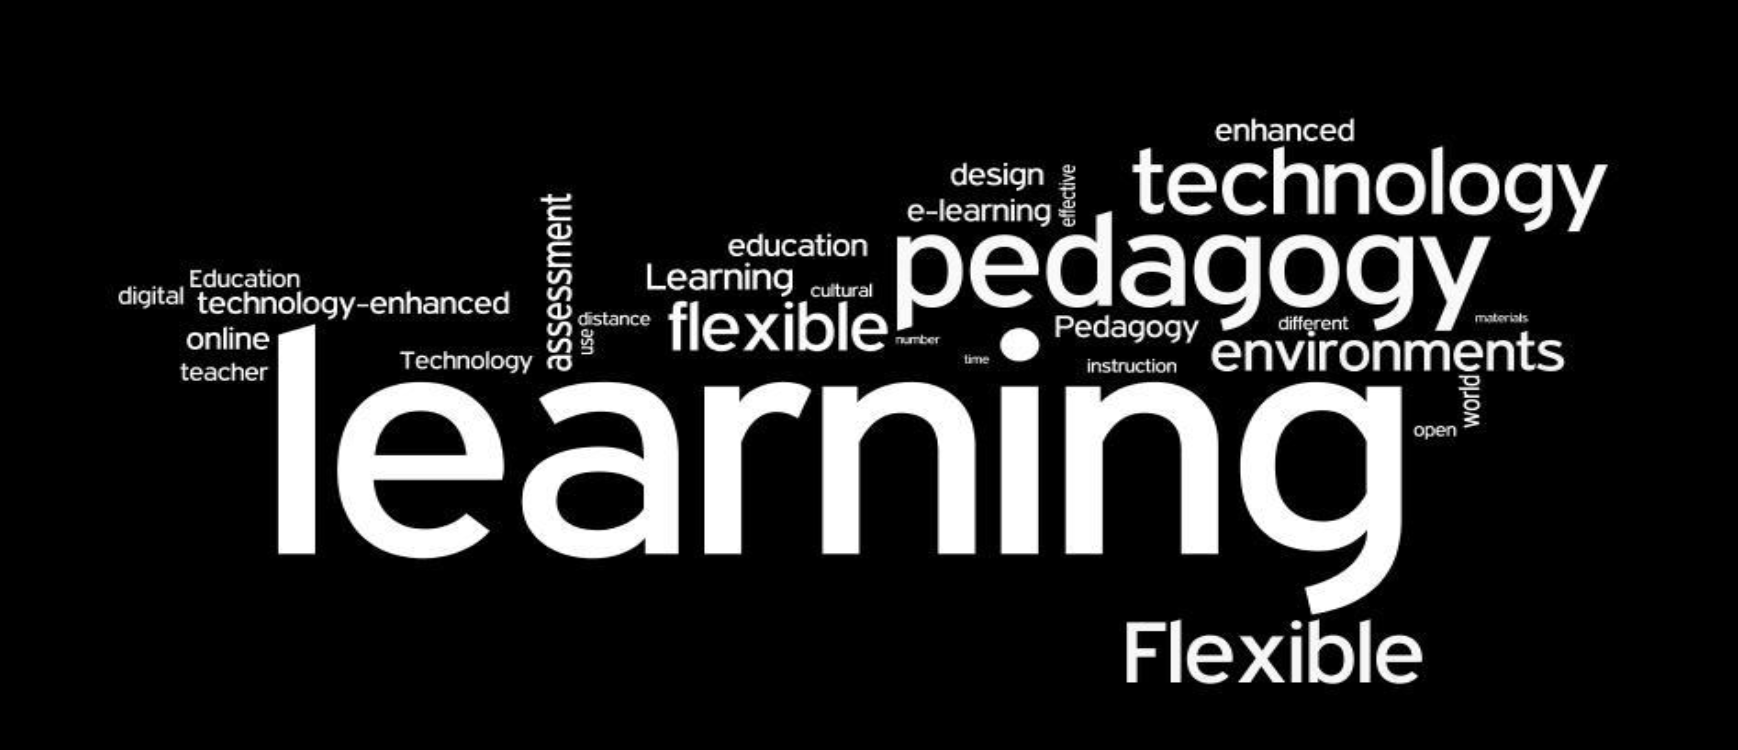
\includegraphics[scale=0.5]{figures/wordCloud}
	\mycaption[Word Cloud Data Visualisation]{Word Cloud Data Visualisation. Figure reproduced from abstracts on flexible learning pedagogies \cite{Gordon2014}.}
	\label{fig:Wordle Word Cloud}
\end{figure}


Kirkpatrick , whilst identifying the disruptive merits of Web 2.0 technology as TEL solutions, identifies \textit{Social Networking} as an established and \textit{Cloud Computing} as an emergent web technology within the context of flexible pedagogies \cite{Burge2011}. Therefore vide the rationale developed thus far this project has opted for a web based "Social Network"  as the envisioned modality for Artemis

Opting for a social network as the modality for implementing Artemis has it's merits:

\begin{enumerate}
    \item Firstly it is cited as a well recognised modality that lends it's self well to flexible pedagogies \cite{Burge2011,Gordon2014}, blended learning strategies  and even the use of participatory learning models (for mapping interaction) \cite{Yager1990,Yager2004} discussed later.
    
    \item It is not unreasonable for both cohort and instructor to emulate the an instructor lead class room environment on a social network. This fulfills the foremost requirement of a successful TEL solution that enables an instructor lead pedagogy, concluded earlier in this chapter.
    
    \item Finally the idea of a social network lends itself well to the need for adapting instructions and course material so as to achieve the best learning outcomes from an instructor lead blended learning approach that uses Artemis i.e. as discussed earlier another hallmark of a successful TEL solution and pedagogy, in conjunction with the need for the blended pedagogy to be instructor lead.
\end{enumerate}

From the perspective of a flexible pedagogy, a social network can empower users by benefiting the \textit{when, where and how}\cite{Gordon2014} of their course delivery. Therefore Artemis may enable the following for implementing a flexible pedagogy \cite{Burge2011}:

\begin{itemize}
    \item \textbf{User Involvement:}
    
    Students may gain greater \textit{flexibility} in deciding \textit{when} to study for W-0, \textit{where} to study for W-0 and \textit{how} to prepare for W-0. Effectively a hypothetical use case could be an international student can prepare W-0 in advance via instructions from a lecturer on Artemis, to help alleviate stress of juggling a move to a new country. Within this context the same student could also identify supplementary learning needs if necessary and even gauge whether this course is a good technical fit for them before investing valuable time and money.
       
    \item \textbf{Collaborative Learning in a Virtual Learning Environment (VLE):}
    
    A VLE suffices to say at this stage, derives functional purpose from it's name and will be explained further in a later section of this chapter. A social network allows for collaborative learning amongst peers enabling a flexible learning methodology \cite{Cubukcuo2012}. Design considerations for this project can also be made to incorporate instructor intervention where necessary \cite{Cubukcuo2012,Burge2011}, without hindering peer  communication and collaboration \cite{Cubukcuo2012}, as may be expected of any popular social network at the time of writing.
    
    There is a plethora of different variants of learning environments that may be incorporated into the design of a VLE \cite{Richmond2005,Cubukcuo2012,Burge2011} which are beyond the scope of this research. However a proactive approach to at least gaining an abstract understanding of these may enhance the quality of learning outcomes by designing an appropriate TEL solution \cite{Cubukcuo2012}; In this case by making design considerations during the development of the network, so that students as well as instructors can interact with each other freely.
    
    This report will focus on the merits and rationale of a \textit{participatory learning model} \cite{Yager1990,Yager2004}, to benefit an understanding of how interaction may be enabled to occur in a social network and ultimately benefit learning outcomes, by considering learner specific needs and adapted instructor intervention \cite{Cubukcuo2012}. This is further discussed in a later section of this chapter and illustrated via possible use cases.
    
\end{itemize}

\label{sec:sec01}
\subsection{Designing and Understanding TEL Solution via Scope of Flexible Pedagogy}
\label{subsec:subsec01}

Flexible pedagogies and learning methodologies focus on improving the \say{when, where and how}, otherwise referred to as the "pace,place and mode" or "degrees of freedom" \cite{Gordon2014}, so as to enable flexible learning towards student benefit. So that the TEL solution this project produces is intuitively an enabler of flexible learning, pedagogy and blended learning that enhances student learning and the UX \cite{Cubukcuo2012,Gordon2014,Team2008}, it may be useful to consider possible design implications via the scope of the aforementioned as illustrated in Figure \textbf{\ref{fig:Flexible Pedagogy Design Considerations for TEL}} \cite{Gordon2014}.As a result of incorporating the degrees of freedom, the ideal position for the result of this project would be towards the top, front-right point of the diagram in Figure \textbf{\ref{fig:Flexible Pedagogy Design Considerations for TEL}}, although the reality is likely to be a compromise.

The following degrees of freedom are identified and their corresponding design implications on this project's TEL solution are considered as follows:

\begin{itemize}[\null]

\item \textbf{Pace}: This degree of freedom broadly refers to the  \say{delivery schedule} \cite{Gordon2014} for the TEL solution and leads to the following design considerations:

\begin{itemize}
\item \textbf{The timing of delivery} is a deployment issue that affects the learning outcomes and pace. Ideally the TEL tool would be made available to students (perhaps circulated via email) before the commencement of W-0. However the tool could also be made available upon commencement of or after W-0, highly contingent on internal policy and approvals vis-a-vis stakeholder appetite.

 It is reasoned that a social network such as Artemis should be intuitively well adapted to the worst case scenario of this issue, as instructions and material are intended to be adapted as per the instructor lead blended learning approach which can be disseminated via the social network as appropriate to the relevant delivery time; flexibly adapting to the the delivery schedule. 
 
 It is disclosed that explicitly determining or influencing the delivery schedule is beyond the reasonable constraints of the project, due to time and logical constraints.

\item \textbf{The scope/size of the curriculum to be delivered} affects pace. As justified earlier, the TEL solution will be designed around an instructor lead methodology and a social network is the preferred modality. The concept of social networks lends itself  well to the idea of dynamically generated as opposed to static course content, at the prerogative of the instructor as per the learning methodology.

Therefore by  designing the social network in a manner that the scope/size of delivery is contingent on the instructor's discretion, this issue is resolved. Furthermore the issue and relevant pedagogical considerations are disclosed in the user manuals ( a deliverable of this project).

\end{itemize}

\item \textbf{Place} : As the name suggests \textit{place} refers to the physical location of user interaction specifically, but also the timing of user interaction as well \cite{Gordon2014}.

\begin{itemize}

\item \textbf{Remote Access} is an inherent design feature of a web based technology, so this this is merely acknowledged and does not require any accommodation in design, as the technical implications of a web technology are obvious in this context.




\item \textbf{Support for Asynchronous and Synchronous Activities \cite{Gordon2014}}: By opting for a design that incorporates blended methodology via a social network, asynchronous and synchronous activities can be supported easily by dynamic web application such as Artemis. Synchronous learning activities can be carried out in a in a class room setting and flexible asynchronous learning on a web based TEL social network lead by the instructor \cite{Gordon2014}.

\end{itemize}

\item \textbf{Mode} : Is an abstract concept that covers the learning technologies,methodologies and pedagogical approach. This overlaps with the previously discussed design consideration, but impresses upon the importance to integrate the aforementioned factors into the design of a TEL tool \cite{Gordon2014} so as to enhance the overall quality of learning outcomes \cite{Cubukcuo2012}.

\begin{itemize}
\item \textbf{Tailored Support}: The need to personalise deliveries according to individual learning requirements is an important aspect of a flexible pedagogy \cite{Gordon2014}. As a design consideration to address this, it is envisioned that  by integrating a participatory learning model \cite{Yager1990,Yager2004} which enables an instructor lead methodology \cite{RickReis,Team2008} delivered via a social network (via comments and posts) to enable instructor-student interaction \cite{Cubukcuo2012}, the need for enabling tailored support is addressed by the nature of the chosen modality.



\item \textbf{Mobile Devices Access}  enhances accessibility enabling a flexible pedagogy \cite{Gordon2014}, by allowing students to choose the mode, place and pace of study. In the past web applications were  developed for computers first and for mobile devices later as an afterthought \cite{W3.CSS2016}. However this has changed with the advent of "mobile first" development and responsive web design \cite{W3.CSS2016}. As a design consideration, it is proposed that a solution operable on a computer should be a minimum viable product (MVP) and responsive web design principles \cite{W3.CSS2016} can be used. However the scope is explicitly limited as this would be beyond the reasonable time and human constraints of the project (it would require mobile testing and a host of development activities that can be reasonable completed before project submission).

However as this is an Open Source project, relevant disclosure for future mobile and responsive web design considerations can be shared via the proposed developer documentation identified later in this report.

\end{itemize}
\end{itemize}



% A single figure
\begin{figure}[H]
	\centering
	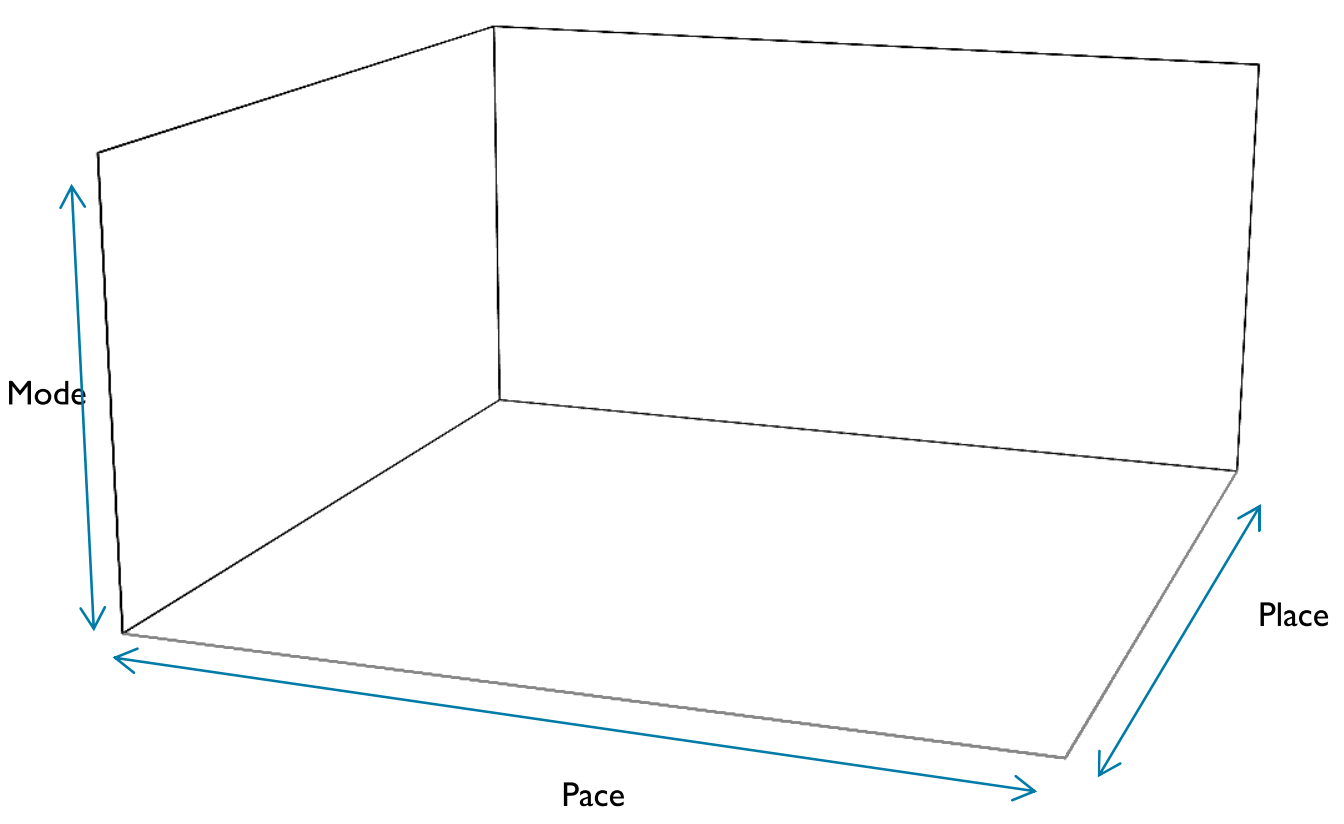
\includegraphics[scale=0.35]{figures/flexibleDesign}
	\mycaption[3D Degrees of Freedom]{Flexible Pedagogy Design Considerations for TEL solution. Figure reproduced from \cite{Gordon2014}.}
	\label{fig:Flexible Pedagogy Design Considerations for TEL}
\end{figure}

\label{sec:sec01}
\subsection{Three Principle Stakeholders}
\label{subsec:subsec01}

Gordon \cite{Gordon2014}, identifies three principle stakeholders within the context of deploying  a TEL solution to enable a flexible pedagogy as illustrated in the following figure. These \textit{principle} stakeholders directly influence the success of a TEL solution designed to enable a flexible pedagogy \cite{Gordon2014}. These principle stakeholders within the context of the project are as follows, for the purpose of stakeholder feedback during the course of the project .

For the purposes of this project, based on the literature \cite{Gordon2014}, the following stakeholders are identified for the purpose of an abstract stakeholder analysis and involvement during the development and evaluation process (It is acknowledged that whilst an extensive stakeholder analysis is desirable it is outside the scope and reasonable constraints of this project):

\begin{itemize}

\item \textbf{System - Institutions}: Are interpreted as the relevant administrative unit of UoB that deal with the application and implication of a TEL solution. This is likely to be the TELED department at the UoB.

\item \textbf{Pedagogical - Teachers}: Instructor values must be identified and considered when designing the tool, to avoid any obvious incompatibilities with pre-dominant pedagogies at the UoB CS department.

\item \textbf{Ontological - Students}: Student values must be identified, as the adoption of the technology and success of the TEL solution, is almost surely contingent on whether or not they are willing to use it.

\end{itemize}

% A single figure
\begin{figure}[H]
	\centering
	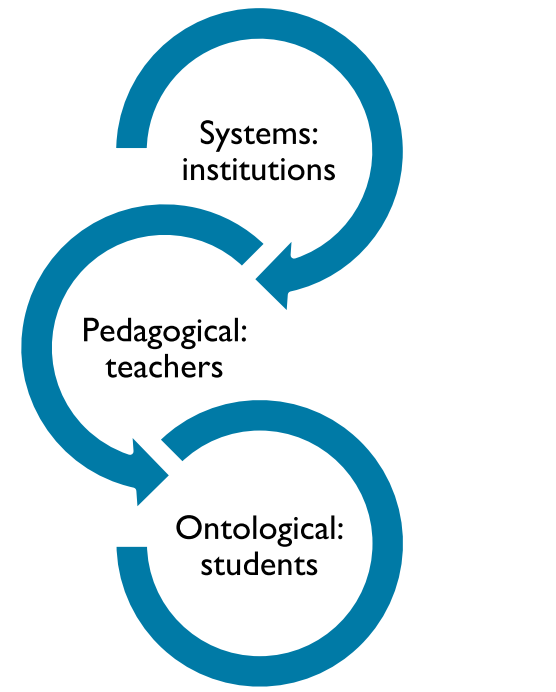
\includegraphics[scale=0.5]{figures/flex}
	\mycaption[Principle Stakeholders- Levels of Flexibility]{Principle Stakeholders- Levels of Flexibility. Figure reproduced from \cite{Gordon2014}.}
	\label{fig:The Three Levels of Flexibility}
\end{figure}

\subsection{Conclusions on Implication of Flexible Pedagogy and Blended Learning Methods on the Creative Design of TEL}
\label{subsec:subsec01}

To summarily amalgamate and draw conclusions on the findings so far; A  web based TEL solution, delivered via the modality of a social network seems to be an  appropriate enabler for a flexible pedagogy and ideal for the purposes of UoB. By intuitively enabling a flexible pedagogy, student users will benefit from flexible learning i.e. greater influence over the pace, place and mode of their education. Effectively by enhancing the aforementioned degrees of freedom, the short comings of W-0 can be overcome by allowing for activities such as tailored feedback, instructor intervention and asynchronous modes of learning.

A social network seem a reasonable vehicle for enabling an instructor lead methodology and will result in a VLE. Interaction via the instructor lead VLE shall be modeled on a participatory learning model, that seeks to enhance the human collaborative learning process \cite{Yager1990,Yager2004}

The next section of this chapter will delve into possible implementations of TEL design focused by the scope of findings so far, considering and proposing possible using possible use cases and criteria for development

\section{Technology Enhanced Learning Solutions}
\label{sec:sec01}

There seems to be no unified definition of TEL, in the literature studied. This project will loosely adhere to the broad definition; \textit { "TEL encompasses all uses of information and communications technologies in learning and teaching"} \cite{Project2009}, interchangeably with concepts such as \textit{e-learning} \cite{Gordon2014}, which is the norm in the literature reviewed. Investigating a concrete definition of TEL, is beyond the scope of this project and despite an ambiguity in the literature it is not deemed problematic for the purposes of development. 

The use of technology in learning is not a recent innovation \cite{Serrano-Laguna2015,TechFacultyinnovate.utexas.edu,Harger1996}. It's proposed implementation over the years are a combination of creativity and research, ranging from TEL via class room clickers \cite{Hatziapostolou2014},  game enhanced learning (GEL) programs \cite{Serrano-Laguna2015,Ibanez2014}, hyper linked interactive books  \cite{Harger1996}, VLE's \cite{Gordon2014,Richmond2005,Burge2011}, Social Networks \cite{Burge2011,Cubukcuo2012} and recently cloud computing \cite{Burge2011} as well.

There is no one "correct" TEL solution out of a wide array of possible implementations, as each are relevant to their own purpose or inspiration. This project  prioritises improved learning outcomes and flexibility for the user. Therefore relevant inspiration from previous implementations will be drawn if compatible with the embedded creative and technical design for the project thus far, prioritising it's purpose over past implementations where in conflict \cite{Burge2011}.

As explained earlier, this project will deliver a web based social network to create a VLE \cite{Gordon2014,Burge2011} adapting features of  participatory learning model \cite{Yager1990,Yager2004} to enable the desired learning methodology and required user interaction within the VLE. By embracing a flexible pedagogy to benefit flexible  and blended learning, the end user's experience and learning outcomes can be improved \cite{Gordon2014,Burge2011}.

The following sections explore the possible use cases (to create a guideline for implementation during development) before concluding the creative design aspect of Artemis by exploring possible interactions between users and underlying rationale.


\subsection{Consideration of Applicable Implementations and Resultant Use Cases}
\label{subsec:subsec01}


Analysing all the previous implementations of TEL are well beyond the reasonable constraints of the project; the possibilities are almost limitless given the creative nature of web technology and social networking. Therefore the following implementations and use cases are considered based on relevance to the underlying objectives and compatability with the creative design of the TEL solution.


    \begin{itemize}[\null]
    \item \subsubsection{Social Network VLEs}
    
    Social networks and web applications have evolved with the advent of Web 2.0 by upgrading users from mere content viewers to creators \cite{Lopez-Vargas2015}. Well known networks such as Facebook and Twitter, allow for various explicit relationships between entities via likes, posts, followers, followers etc \cite{Lopez-Vargas2015}. Most relevant to the purpose of this project social networks intuitively create an opportunity to collaboratively learn and even contribute to enhance existing learning resources\cite{Lopez-Vargas2015,Magnisalis2011}. This natural synergy may lend itself well to the idea of instructor lead learning, participatory/collaborative interaction based learning models via the inherent design of a generic social network; Therefore this project will encourage a creative design for the social network that enables prompts from instructors (via posts, comments, personal messages and likes etc) for the purpose of an adaptable and instructor lead approach, as well as collaboration between all users to create a richer VLE.
    
    Maginisalis et al \cite{Magnisalis2011} analysed TEL from the perspective of system planning, generally the broad subject matter of  Adaptive Education Systems (AES) and specifically it's two sub-sets adaptive and intelligent systems   for \textit{collaborative learning}; Collectively referred to as Adaptive and/or Intelligent Collaborative Learning Support Systems (AICLS).
    
    This project will adapt concepts from an adaptive (not intelligent) learning environment, to encourage collaborative learning as it supports participatory and instructor lead approaches to learning \textbf{that can be adapted}.  A social network that enables an AES may encourage  collaboration between users within the aforementioned context; Possible use cases are identified within a classification system for AICLS  by Maginisalis et al, which encourages analysis within the following dimensions\cite{Magnisalis2011}:
    
    \begin{enumerate}
        \item Pedagogical objective (PO): The underlying PO of the system has already been explained in depth. However to highlight the inherent capabilities of a social network that may encourage collaboration and participation amongst users (instructor and student) via a use case; The proposed social network may enable  asynchronous conversation via \textit{posts, comments or messages} between instructors and students and subesquent  personalised user feedback via comments and likes. This may  allow for retrospective evaluation of the learning environment to be adapted as necessary (commenting further to elaborate/clarify, re-reading generated content, deleting or creating a new posts).
        
        \item Target of Intervention (TI): In a very abstract sense (to remain withing project constraints), refers to what is being adapted by an AICLS. It is proposed that this project allow for the creation and adaption of instructions and learning materials via the use of posts and commentary, by allowing instructor intervention where students are collaborating to learn. This would allow for an enrichment of the VLE via user collaboration \cite{Lopez-Vargas2015}, tempered by the instructors prompts via a participatory learning model \cite{Yager1990} as part of an instructor lead blended learning strategy. E.g. Students are asked to share thoughts on subject matter collaboratively, thus enriching the VLE, but ultimately tempered by an instructor lead methodology adapted for the purposes of enriching the VLE resources (i.e. past posts and commentary).
        
        \item Modeling and Technology : Within the context of this project it refers to how models intimately affect the overall design and resultant usage of technology. To enable collaborative learning within an instructor lead methodology it is proposed that the social network is designed in a manner that it allows for the intuitive use of an adapted participatory learning model \cite{Yager1990,Yager2004} . Furthermore within the context of this dimension, it must be highlighted that Web 2.0 technology allows for user content to enhance learning resources and encourage user collaboration, further cementing the rationale for building a Web Application .
        
        \item Design space (DS): This has to do with the modality of the TEL tool and how it enables collaborative learning between users (implicitly and explicitly); as such it is an abstract dimension, subject to interpretation via the scope of architectures/models and pedagogies embedded within the Social Network. It suffices to surmise that the entirety of this research is bound to directly/indirectly affect the DS. Subject to the constraints of this project analysis of further models and architectures have been ignored.
    \end{enumerate}
    
    \item \subsubsection{Crowd Sourcing and OER}
    OER is an acronym for \textit{open educational resources} i.e. a free and openly licensed educational material for teaching, learning and other purposes. It is an emergent trend in TEL implementations and has garnered the support of various social organisations such as the OECD and UNESCO \cite{UNESCO,CreativeCommons}, due to it's potential for positive social contributions via easy and flexible dissemination and adoption by third parties.
    
    This trend is reminiscent of the Open Source Software movement and seems to have been inspired by it, as indicated by one of the many available working definitions "Open Educational Resources are teaching and learning materials that you may freely use and reuse, without charge. OER often have a Creative Commons or GNU license that state specifically how the material may be used, reused, adapted, and shared" \cite{CreativeCommons}.
    
    Crowd Sourcing is also a relatively young trend, which has been successful within the context of generating rich learning environments via social networking, such as in the cases of Wikiepedia and wikis. It has been proposed in recent research that OER's could make use of crowd sourcing to generate flexible and rich learning resources, particularly within the context of specialist STEM OER's \cite{Hills2015,Estelles-Arolas2012}. Therefore this project has sought inspiration from this proposed implementation by trying to create a VLE via social network, that is improved over time via collaborative/participatory learning and an instructor lead methodology; Via intervention from instructor and students.
    
    Given the parallels between  OER and Open Source software, it is believed that it would be a prudent design consideration to make the TEL solution open source with the view of future scalability. The tool can be developed and disseminated with the view of being shared as an OER's platform to allow collaboration between instructors, students and third parties i.e. users from other courses or potentially even other schools. If this works it could hypothetically crowd source future development and inspiration to evolve the solution in the spirit of a truly adaptive learning environment.
    
    It can be reasonably argued that an Open Source solution might potentially be useful for future creative endeavours by faculty/cohort members wishing to adapt the source code for their own purposes. Therefore detailed developer documentation will be provided for the purposes of Artemis; aligning with generally accepted best practice for Open Source projects.
    
    
    The following can now be surmised before concluding this section:
    \begin{itemize}
        \item Open Source \& OER: This project can and  will be disseminated as an Open Educational Resource so as to enable future scalability and encourage others to reuse this code as appropriate towards their own needs. At it it's simplest form this would imply an appropriate legal modality for open dissemination in the public domain \cite{UNESCO}. For the purposes of this project it will be implemented via detailed developer documentation (See page \textbf{ \pageref{devDocPage}} or \url{https://github.com/TaimurAhmed/summerProject2017/wiki}).
        
        \item Crowd Sourcing: As discussed earlier the selected modality for this TEL solution is envisaged as social network because it seems to be a natural enabler for the desired learning methodology, pedagogy and lends itself well to the concept of an Adaptive VLE system. Given the inherent nature of mainstream social networks, this project has aimed to allow for crowd sourced knowledge via teacher and cohort interaction. This aspiration is further elaborated upon in the next section on Particpatory Learning model via a proposed \textit{use case}, after deployment.
    \end{itemize}
    
    
    \item \subsubsection{Participatory Learning Model}
    \label{participatoryLearningModel}
 
    Yager's \cite{Yager1990,Yager2004,Yager2004a} extensive work on participatory learning models and paradigms provides an interesting perspective, seeking to improve our understanding of the  complex human learning process and embed it in digital design of products, systems and software; To improve neural network learning in a manner analogous to human collaborative learning, the latter of which is applicable and adaptable for this project. The participatory learning paradigm has been explicitly designed by Yager \cite{Yager2004,Yager2004a} to be complimentary towards other learning models and be flexibly applicable for enhancing technologies in various contexts.
    
    To remain within the constraints of this project, abstract concepts are adapted to explain and design, the social network's user interaction so as to enable instructor lead \textit{participatory} learning; By inspiring the design of the social network. The crux of Yager's research addresses the need to introduce \textbf{independent critics} \cite{Yager2004a,Yager2004,Yager1990}, so as to temper an individual/group's beliefs and observation system \cite{Yager1990} to improve the overall  process; strongly reminiscent of an instructor lead pedagogy that is adaptive i.e. the best pedagogy for implementing a TEL solution that is beneficial for learning (See section \textbf{\ref{embeddingBestPracticePedagogy}}).
    
    The following illustrate Yager's participatory model and a possible adaptation upon which to model the implementation of Artemis:


\begin{figure}[H]
	\centering
	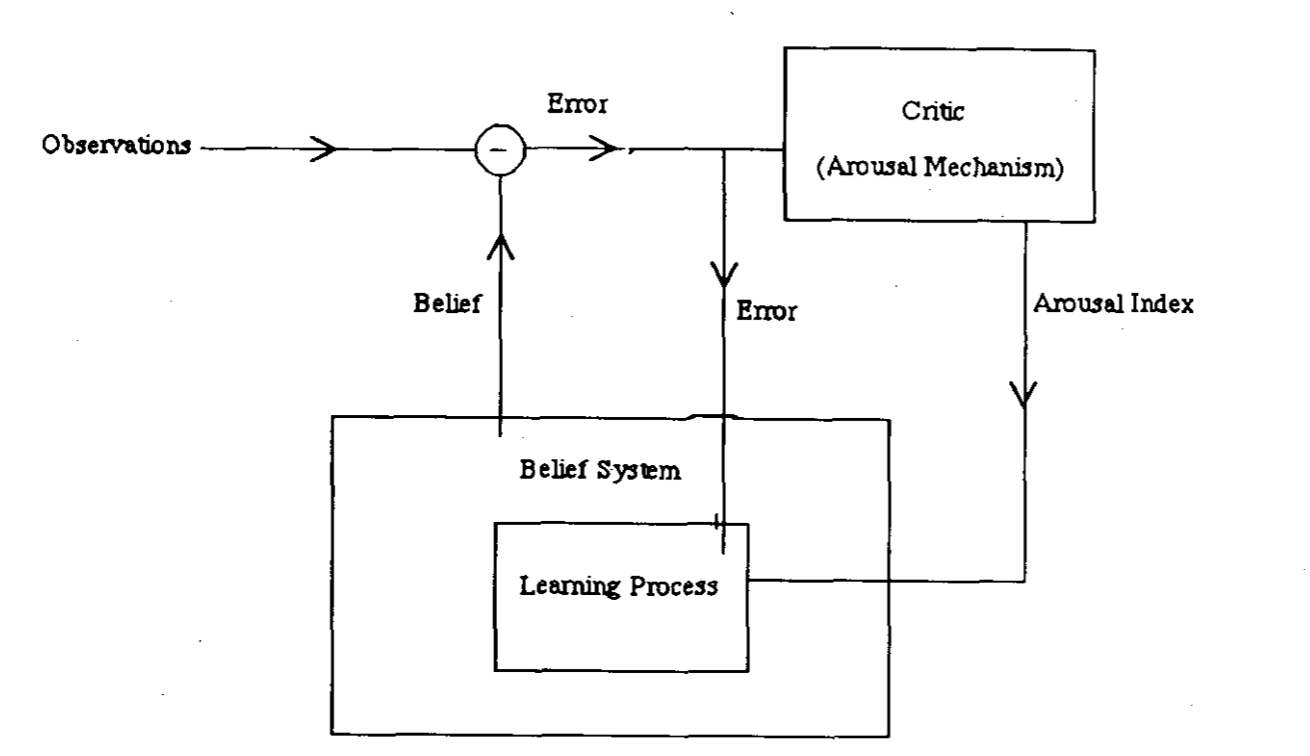
\includegraphics[scale=0.5]{figures/particip}
	\mycaption[A Participatory Learning Process,to Enrich Belief System and Tempered by Critic]{A Participatory Learning Process,to Enrich Belief System and Tempered by Critic \cite{Yager1990}.}
	\label{fig:Relationship Between Learning Process,Belief System and Critic}
\end{figure}

\newpage

\begin{figure}[H]
	\centering
	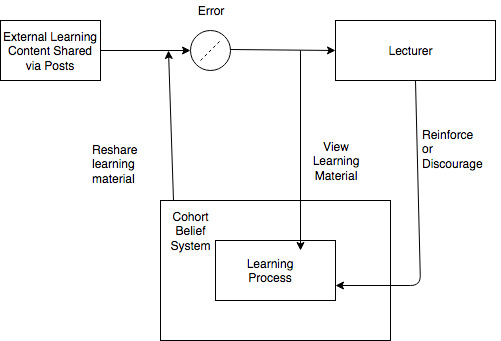
\includegraphics[scale=0.5]{chapters/chapter02/figures/useCase.jpg}
	\mycaption[Illustration of  Use Case, depicting possible adaptation of Participatory Learning Model to Proposed Social Network]{Illustration of  Use Case, depicting possible adaptation of Participatory Learning Model to Proposed Social Network}
	\label{fig:UseCaseParticipatory}
\end{figure}


    The core concepts of Yager's proposals can intuitively be adopted into a social network as depicted by the two contrasting figures above and further explained as follows:
    \begin{itemize}
        \item It is reasonable to assume that a social network can be used to share new academic resources, discuss existing ones and explain various course content material via interaction within the cohort; effectively creating a belief system within which the CS cohorts collaboratively learn from each other. It can also be reasonably argued that a lecturer can serve as the independent moderator or critic. It can be reasoned that instructors who are independent of a student's belief of what is correct/incorrect within the context of the course material (as they are experts) may intervene to promote or discourage influences on the belief system that affect learning. E.g. If a student shares an online tutorial that is sub-standard and may cause an undesirable effect on the cohort's belief system (i.e. the cohort may start to believe the tutorial is worth investing time in), the independent moderator may intervene to discourage the hypothetical educational resource. Alternatively if the tutorial shared is deemed useful or relevant, lectures may use their position to positively influence and embed the learning material in the cohort's belief system (See page \textbf{\pageref{fig:UseCaseParticipatory}} for implementation in Artemis and further illustration).
        
        Effectively these use cases resonates well with the introduced concepts of adaptive VLE's implemented through the modality of social netwrok, where good academic values are reinforced by peers in a collaborative environment and tempered my independent mediators. Furthermore this also resonates with the idea of a self enriching solution which crowd sources academic sources of information and is compatible with an instructor lead flexible pedagogy that uses adaptable instruction material.
    \end{itemize}
    

    
    \end{itemize}
    
\section{Chapter Conclusion}

To conclude this chapter the following points are summarised and have been used to inspire, design and implement the proposed TEL solution:

\begin{itemize}

    \item An underlying pedagogical strategy that is instructor lead and allows for adaptation of instruction material is compatible with TEL solutions that genuinely enhance learning and/or teaching outcomes (Section \ref{}). Artemis will seek to enable this strategy during implementation.
    
    \item The TEL solution is to be designed as a social network because it is an enabler for flexible pedagogies and instructor lead teaching; Benefiting users by improving the flexibility for the when, where and how (\textit{pace,place and mode}) of learning .
    
    \item The UoB, instructors and students have been identified as the key stakeholders of this project due their relationship with flexible pedagogical solutions; So their views  and values will be incorporated into the implementation of the project via stakeholder analysis, interaction and evaluation.
    
    
    \item A social network is desirable because it is easy to envision an adaptive and self enriching VLE that can improve over time; resonating with the concept of adaptive instructor lead pedagogies and tools.
    
    \item To give further credence to the assertion of adaptive, use cases via the lens of participatory learning and independent moderators that affect the learning process will be considered during implementation.
    
    \item Finally the social network will be disseminated as an OER with appropriate licensing and  developer documenation support; Ensuring a VLE that can be used by other parties and adapted (\textit{forked via Github}) for their own purposes or scaled up over time.
    
\end{itemize}

    
    
    
    